\documentclass{article}

%Linux command prompt showing package
\usepackage{listings,menukeys}

%Page format
\usepackage{pdfpages,fancyhdr}
\usepackage[margin=1in]{geometry}

%Math packages and custom commands
\usepackage{algpseudocode,amsmath,framed,tikz,sans,mathtools,amsthm,enumitem,amssymb,dsfont,tabularray,fancyvrb}
\usepackage[short]{optidef}
\usepackage[hidelinks]{hyperref}
\usepackage[table,xcdraw]{xcolor}
%\usepackage[labelformat=empty]{caption}
\usepackage[utf8]{inputenc}
\usetikzlibrary{arrows.meta}
\usepackage[TABcline]{tabstackengine}
\TABstackMath


\usepackage[table]{xcolor}
\usepackage{collcell}
\usepackage{hhline}
\usepackage{pgf}
\usepackage{multirow}

\def\colorModel{hsb}
\newcommand\ColCell[1]{
	\pgfmathparse{#1<50?1:0}  %Threshold for changing the font color into the cells
	\ifnum\pgfmathresult=0\relax\color{white}\fi
	\pgfmathsetmacro\compA{0}      %Component R or H
	\pgfmathsetmacro\compB{#1/100} %Component G or S
	\pgfmathsetmacro\compC{1}      %Component B or B
	\edef\x{\noexpand\centering\noexpand\cellcolor[\colorModel]{\compA,\compB,\compC}}\x #1
} 
\newcolumntype{E}{>{\collectcell\ColCell}m{0.4cm}<{\endcollectcell}}  %Cell width
\newcommand*\rot{\rotatebox{90}}

%Course Info
\newcommand{\coursenumber}{ECE421}
\newcommand{\coursename}{\coursenumber: Introduction to Machine Learning}
\newcommand{\courseyear}{2024}
\newcommand{\coursesemester}{Fall}
\newcommand{\coursefullname}{\coursename~---~\coursesemester~\courseyear}
%Handout Info
\newcommand{\haname}{}
\newcommand{\hatypeandnun}{Worksheet 1 Solution: Pocket Algorithm and Linear Regression}


\DeclareMathOperator{\R}{\mathbb{R}}
\newcommand{\probP}{\mathds{P}}
\DeclareMathOperator{\E}{\mathbb{E}}
\DeclareMathOperator{\Var}{\text{Var}}
\DeclareMathOperator{\Cov}{\text{Cov}}
\renewcommand{\arraystretch}{1.3}
\newcommand{\norm}[2][2]{\| #2\|_{#1}}

\newcommand{\notp}{\neg p}
\newcommand{\notq}{\neg q}
\newcommand{\notr}{\neg r}
\newcommand{\notP}{\neg P}
\newcommand{\notQ}{\neg Q}

\newcommand{\setD}{\mathcal{D}}
\newcommand{\setR}{\mathbb{R}}
\newcommand{\setRd}{\mathbb{R}^d}
\newcommand{\setRdone}{\mathbb{R}^{d+1}}
\renewcommand{\vec}[1]{\underline{#1}}
\newcommand{\vecw}{\vec{w}}
\newcommand{\vecx}{\vec{x}}
\newcommand{\vecy}{\vec{y}}
\newcommand{\vecxn}{\vec{x}_n}
\newcommand{\setxnyn}{\left\{(\vecxn, y_n)\right\}_{n=1}^{N}}


\newcommand{\con}{\wedge}
\newcommand{\dis}{\vee}
\newcommand{\false}{\text{F}}
\newcommand{\terue}{\text{T}}

% verbatim
\DefineShortVerb{\|}
\SaveVerb{py}|Python|
\SaveVerb{num}|NumPy|
\SaveVerb{sci}|scikit-learn|
\SaveVerb{tp1}|test_Part1()|
\SaveVerb{tp2}|test_Part2()|

\definecolor{shadecolor}{gray}{0.9}

\theoremstyle{definition}
\newtheorem*{answer}{Answer}
\newcommand{\note}[1]{\noindent{[\textbf{NOTE:} #1]}}
\newcommand{\hint}[1]{\noindent{[\textbf{HINT:} #1]}}
\newcommand{\recall}[1]{\noindent{[\textbf{RECALL:} #1]}}
\newcommand{\remark}[1]{\noindent{[\textbf{REMARK:} #1]}}
\newcommand{\expect}[1]{\noindent{[\textbf{What we expect:} #1]}}
\newcommand{\mysolution}[1]{\noindent{\begin{shaded}\textbf{Your Solution:}\ #1 \end{shaded}}}

\newlist{question}{enumerate}{3}
\setlist[question, 1]{label=\Large \textbf{Q\arabic{questioni}}, leftmargin=\parindent, rightmargin=10pt}
\setlist[question, 2]{label=\large \textbf{\arabic{questioni}.\alph{questionii}}, leftmargin=15pt, rightmargin=15pt}
\setlist[question, 3]{label=\textbf{\arabic{questioni}.\alph{questionii}.\kern1.5pt\roman{questioniii}},	leftmargin=30pt, rightmargin=30pt}

\newlist{todolist}{itemize}{2}
\setlist[todolist]{label=$\square$}
\usepackage{pifont}
\newcommand{\cmark}{\ding{51}}%
\newcommand{\xmark}{\ding{55}}%
\newcommand{\done}{\rlap{$\square$}{\raisebox{2pt}{\large\hspace{1pt}\cmark}}%
	\hspace{-2.5pt}}
\newcommand{\wontfix}{\rlap{$\square$}{\large\hspace{1pt}\xmark}}


\title{\vspace{-2.5cm}\textbf{\coursefullname}\\\hatypeandnun\\\haname}
\date{}

%\chead{}
\rhead{\haname}
\lfoot{}
\cfoot{\coursenumber~\coursesemester~\courseyear~---~\hatypeandnun}
\rfoot{\thepage}
\renewcommand{\headrulewidth}{0.4pt}
\renewcommand{\footrulewidth}{0.4pt}
\pagestyle{fancy}
\setlength{\parindent}{0pt}

% NOTE(joe): This environment is credit @pnpo (https://tex.stackexchange.com/a/218450)
\lstnewenvironment{algorithm}[1][] %defines the algorithm listing environment
{   
	\lstset{ %this is the stype
		mathescape=true,
		frame=tB,
		numbers=left, 
		numberstyle=\tiny,
		basicstyle=\rmfamily\scriptsize, 
		keywordstyle=\color{black}\bfseries,
		keywords={,procedure, div, mod, for, to, input, output, return, datatype, function, in, if, else, foreach, while, begin, end, } %add the keywords you want, or load a language as Rubens explains in his comment above.
		numbers=left,
		xleftmargin=.04\textwidth,
		#1 % this is to add specific settings to an usage of this environment (for instnce, the caption and referable label)
	}
}
{}

\begin{document}

\maketitle
\vspace*{-2cm}
\section*{Notation}
\begin{enumerate}[label=(\alph*)]
	\item We use a \textbf{underline} to represents \textbf{column vectors}, \textit{e.g.}, $\vec{p} \in \setR^{k}$ represents a column vector with $k$ elements. We adopt the following notations to list the elements of a \textbf{column vector} $$\vec{p} = (p_1, p_2, \ldots, p_k)=\begin{bmatrix}
		p_1\\
		p_2\\
		\vdots\\
		p_k
	\end{bmatrix}.$$ Note the usage of parentheses and brackets. The notation with parentheses provides a more compact representation of vectors and optimizes space usage.\\
	Additionally, \textbf{row vectors} can be represented by $\vec{q}^\top = \left[p_1, p_2, \ldots, p_k\right]$. Note the use of transpose and brackets.\\ Finally, the context and notation should make it clear whether a vector is a column vector or a row vector.
	\item For all questions we denote the weight vector by $\vecw=(b, w_1, \ldots, w_d) \in \setRdone$, where $b \in \mathbb{R}$ is the bias term, and we denote the example vectors by $\vecx=(1, x_1, x_2, \ldots, x_d) \in \setRdone.$
	\item In the following, LFD refers to the textbook ``Learning from Data.''
\end{enumerate}
 
\begin{question}[start=0]
	\item \textbf{Linear Algebra Review}
	\begin{question}
		\item \textbf{(The \( \ell_p \)-norm)} For a real number \( p \geq 1 \), define the \( \ell_p \)-norm of a vector \( \vec{x} \in \mathbb{R}^n \).
		\begin{answer}
			To answer this question, please review your notes for the linear algebra course or any introductory linear algebra textbook.
		\end{answer}
		\item \textbf{(The \( \ell_1 \), \( \ell_2 \), and \( \ell_\infty \)-norm)} Consider the vector $\vecx = (5,2,-3)$. Find the \( \ell_1 \), \( \ell_2 \), and \( \ell_\infty \)-norm of $\vecx$.
		\begin{answer}
			~
			\begin{itemize}
				\item $\ell_1$-norm: $\mid5\mid + \mid2\mid + \mid-3\mid = 10$
				\item $\ell_2$-norm: $\sqrt{5^2 + 2^2 + (-3)^2} = \sqrt{38}$
				\item $\ell_\infty$-norm: $\max(\mid5\mid, \mid2\mid, \mid-3\mid) = 5$
			\end{itemize}
		\end{answer}
		\item \textbf{(Matrix Multiplication)} Let $\vecw=(w_0, w_1, \ldots, w_d)$ and $\vec{x}_i=(x_{i0}, x_{i1}, \ldots, x_{id})$ for $i \in \{1, 2, \ldots, N\}$. Let   
		\begin{align*}
			X &= \begin{bmatrix}
				x_{10} & x_{11} & \dots & x_{1d} \\
				x_{20} & x_{21} & \dots & x_{2d} \\
				\vdots & \vdots & \dots & \vdots \\
				x_{N0} & x_{N1} & \dots & x_{Nd}
			\end{bmatrix}=\begin{bmatrix}
				\vecx_{1}^\top \\
				\vecx_{2}^\top \\
				\vdots \\
				\vecx_{N}^\top
			\end{bmatrix},\\
			\vec{\hat{y}} &= \begin{bmatrix}
				\hat{y}_1 \\
				\hat{y}_2 \\
				\vdots \\
				\hat{y}_N
			\end{bmatrix} = \begin{bmatrix}
				\vecw^\top \vecx_{1} \\
				\vecw^\top \vecx_{2} \\
				\vdots \\
				\vecw^\top \vecx_{N}
			\end{bmatrix}.
		\end{align*}
		Show that $\underline{\hat{y}} = X\vecw$.
		\begin{answer}
			To answer this question, please review your notes for the linear algebra course or any introductory linear algebra textbook.
		\end{answer}
	\end{question}
	\item \textbf{Gradient and Optimization Fundamentals}
	\begin{question}
		\item \textbf{(Gradient)} Prove that $\nabla_{\!\vecx}(\vec{a}^\top \vecx) = \vec{a}$, and $\nabla_{\!\vecx}(\vec{x}^\top \vec{a}) = \vec{a}$ and $\nabla_{\!\vecx}(\vecx^\top A \vecx)=2A\vecx$, where $\vec{a}$ and $\vecx$ are vectors with $k$ entries and $A$ is a symmetric squared matrix.
		\begin{answer}
			 We prove that $\nabla_{\!\vecx}(\vecx^\top A \vecx)=(A+A^\top)\vecx$, for any square matrix $A$. Observe that $\vecx^\top A \vecx = \sum\limits_{i=1}^{k}  x_i \sum\limits_{j=1}^{k} A_{i,j} x_j$. Hence, for any $t \in \{1, 2, \ldots, k\}$,
			\begin{align*}
				{\frac {\partial }{\partial x_t}}(\vecx^\top A \vecx)  &= {\frac {\partial }{\partial x_t}}(\sum\limits_{i=1}^{k}  x_i \sum\limits_{j=1}^{k} A_{i,j} x_j) = {\sum\limits_{i=1}^{k}\frac {\partial }{\partial x_t}(x_i \sum\limits_{j=1}^{k} A_{i,j} x_j)}\\
				&= \sum\limits_{i=1}^{k}\left((\frac {\partial }{\partial x_t}x_i)(\sum\limits_{j=1}^{k} A_{i,j} x_j) + x_i \frac {\partial }{\partial x_t}(\sum\limits_{j=1}^{k} A_{i,j} x_j)\right)\\
				&= {\sum\limits_{i=1}^{k}(\frac {\partial }{\partial x_t}x_i)(\sum\limits_{j=1}^{k} A_{i,j} x_j)} + \sum\limits_{i=1}^{k} x_i \frac {\partial }{\partial x_t}(\sum\limits_{j=1}^{k} A_{i,j} x_j)\\
				&= {\sum\limits_{j=1}^{k} A_{t,j} x_j} + \sum\limits_{i=1}^{k} x_i A_{i, t}.
			\end{align*}
			Therefore, 
			\begin{align*}
				\nabla_{\!\vecx}(\vecx^\top A \vecx) &= \begin{bmatrix}
					{\frac {\partial }{\partial x_1}}(\vecx^\top A \vecx)\\
					{\frac {\partial }{\partial x_2}}(\vecx^\top A \vecx)\\
					\vdots\\
					{\frac {\partial }{\partial x_k}}(\vecx^\top A \vecx)
				\end{bmatrix} = \begin{bmatrix}
				{\sum\limits_{j=1}^{k} A_{1,j} x_j} + \sum\limits_{i=1}^{k} x_i A_{i, 1}\\
				{\sum\limits_{j=1}^{k} A_{2,j} x_j} + \sum\limits_{i=1}^{k} x_i A_{i, 2}\\
				\vdots\\
				{\sum\limits_{j=1}^{k} A_{k,j} x_j} + \sum\limits_{i=1}^{k} x_i A_{i, k}
				\end{bmatrix} = \begin{bmatrix}
				{\sum\limits_{j=1}^{k} A_{1,j} x_j}\\
				{\sum\limits_{j=1}^{k} A_{2,j} x_j}\\
				\vdots\\
				{\sum\limits_{j=1}^{k} A_{k,j} x_j}
				\end{bmatrix} + \begin{bmatrix}
				\sum\limits_{i=1}^{k} x_i A_{i, 1}\\
				\sum\limits_{i=1}^{k} x_i A_{i, 2}\\
				\vdots\\
				\sum\limits_{i=1}^{k} x_i A_{i, k}
				\end{bmatrix} \\
				&= A \underline{x} + A^\top \underline{x} = (A + A^\top) \underline{x}.
			\end{align*}
			Thus, $\nabla_{\!\vecx}(\vecx^\top A \vecx) = (A + A^\top) \underline{x}$. When $A$ is symmetric, $\nabla_{\!\vecx}(\vecx^\top A \vecx) = 2A\underline{x}$.
		\end{answer}
		\item \textbf{(Exercise 3.17 (a),(b) in LFD)} Recall that for a scalar-valued function $f : \mathbb{R}^n \to \mathbb{R}$ and a vector $\underline{p} \in \mathbb{R}^n$, the first-order Taylor series approximation of $f(\vecx + \vec{p})$ is $f(\vecx + \vec{p}) \approx f(\vecx) + \nabla f(\vecx)^\top \vec{p}$. Consider the function $E(u, v) = e^u + e^{2v} + e^{uv} + u^2 - 3uv + 4v^2 - 3u - 5v$, where $u$ and $v$ are scalars.
		
		\begin{question}
			\item Denote by $\hat{E}_1(\Delta u, \Delta v)$ the first-order Taylor series approximation of $E$ at $(u, v) = (0, 0)$. We know that $\hat{E}_1(\Delta u, \Delta v)$ is of the form $\hat{E}_1(\Delta u, \Delta v) = a_u \Delta u + a_v \Delta v + a$. What are the values of $a_u$, $a_v$, and $a$?
			\begin{answer}
				Observe that $\nabla E (u,v) = \begin{bmatrix}
					{\frac {\partial }{\partial u}} E (u,v) \\
					{\frac {\partial }{\partial v}} E (u,v)
				\end{bmatrix} = \begin{bmatrix}
				e^u+ve^{uv}+2u-3v-3 \\
				2e^{2v} + u e^{uv} - 3v +8v-5
				\end{bmatrix}$. Hence, by the first-order Taylor series approximation of $E$ at $(0,0)$,
				\begin{align*}
					E\left(\underline{0} + (\Delta u, \Delta v)\right) \approx E(\underline{0}) + \nabla E(\underline{0})^\top (\Delta u, \Delta v) = 3 + (-2, -3)^\top (\Delta u, \Delta v) = 3 -2\Delta u - 3\Delta v,
				\end{align*}
				Thus, $a_u = -2, a_v = -3$, and $a=3$.
			\end{answer}
			
			\item Minimize $\hat{E}_1$ over all possible $(\Delta u, \Delta v)$ such that $\|(\Delta u, \Delta v)\|_2 = 0.5$, \textit{i.e.},
			\begin{mini*}
				{\Delta u, \Delta v}{\hat{E}_1(\Delta u, \Delta v)}
				{}{}
				\addConstraint{\|(\Delta u, \Delta v)\|_2}{ = 0.5.}
			\end{mini*}
			Recall that the column vector $(\Delta u^* , \Delta v^* )$ that minimizes $\hat{E}_1$ is in the direction of $-\nabla E(u, v)$, \textit{i.e.}, the negative gradient direction. Compute $(\Delta u^* , \Delta v^* )$ that minimizes $\hat{E}_1$, and the resulting $\hat{E}_1(\Delta u^*, \Delta v^*)$.
			\begin{answer}
				Note that 
				\begin{align*}
					\hat{E}_1(\Delta u, \Delta v) = 3 + (-2, -3)^\top (\Delta u, \Delta v) = 3 + \|(-2, -3)\|_2 \|(\Delta u, \Delta v)\|_2 \cos{\theta}, 
				\end{align*}
				where $\theta$ is the angle between the two vectors $(-2, -3)$ and $(\Delta u, \Delta v)$. Hence, the vector $(\Delta u, \Delta v)$ with $\|(\Delta u, \Delta v)\|_2 = 0.5$ that minimizes $\hat{E}_1$ must be in the opposite direction of $(-2, -3)$, \emph{i.e.}, $\cos{\theta}=-1$. Therefore, $(\Delta u^*, \Delta v^*) = -0.5 \frac{(-2, -3)}{\|(-2, -3)\|_2} = \frac{(2, 3)}{2\sqrt{13}}$.\footnote{Note that $(-2, -3)$ is in fact $\nabla E(\underline{0})$ and $(\Delta u^*, \Delta v^*)$ must be in the opposite direction of $\nabla E(\underline{0})$.}
			\end{answer}
		\end{question}
	\end{question}
	\item \textbf{(Perceptron Learning Algorithm)}	Given a dataset $\setD=\setxnyn$, where $\vecxn \in \setRd$ and $y_n \in \{+1, -1\}$, we wish to train a Perceptron model
	\begin{equation*}
		h(\vecx) = \text{sign}\left(b + \sum_{i=1}^d w_i x_i \right) = \text{sign}(\vecw^\top \vecx)
	\end{equation*}
	that correctly classifies \textit{all} examples in $\setD$. Consider the perceptron weight update rule
	\begin{equation*}
		\vecw(t+1) = \vecw(t) + y_n\vecxn,
	\end{equation*}
	where $(\vecxn, y_n)$ is the misclassified datapoint after iteration $t$. This weight update rule moves the weights in the direction of classifying examples correctly. To see
	this, show the following.
	\begin{question}
		\item If $\vecx(t)$ is misclassified by $\vecw(t)$, show that $y_n\vecw^\top(t)\vecxn \leq 0$.
		\begin{answer}
			When  $\vecx(t)$ is misclassified, we must have one of the following cases.
			\begin{itemize}
				\item $\vecw^\top(t)\vecxn = 0$.\footnote{The Perceptron model identifies any point on the decision boundary as a misclassification.}
				\item $\vecw^\top(t)\vecxn > 0$ but $y_n = -1$.
				\item $\vecw^\top(t)\vecxn < 0$ but $y_n = +1$.
			\end{itemize}
			 Observe that in the above cases, $y_n\vecw^\top(t)\vecxn \leq 0$.
		\end{answer}
		\item Use the equation for $\vecw(t+1)$ to show that $y_n\vecw^\top(t+1)\vecxn > y_n\vecw^\top(t)\vecxn$.
		\begin{answer}
			\begin{align*}
				y_n\vecw^\top(t+1)\vecxn = y_n(\vecw(t) + y_n\vecxn)\vecxn = y_n\vecw(t)\vecxn + (y_n)^2\vecxn\vecxn = y_n\vecw(t)\vecxn + \|\vecxn\|_2^2 > y_n\vecw(t)\vecxn,
			\end{align*}
			where the last inequality is due to the fact that $\|\vecxn\|_2^2 > 0$  since $x_{n,0}=1$.
		\end{answer}
		\item Argue that the weight update from $\vecw(t)$ to $\vecw(t+1)$ is a move ``in the right direction."
		\begin{answer}
			Note that we eventually want a weight vector that  can successfully classify $\vecxn$, \textit{i.e.}, we want $y_n\vecw~\vecxn$ to be positive. By updating $\vecw$ according to the Perceptron weight update rule, we make $y_n\underline{w}~\vecxn$ more positive. Therefore, this is a move ``in the right direction." 
		\end{answer}
	\end{question}
	\remark{Problem 1.3 in LFD, page 33, shows steps towards a rigorous proof of convergence of the Perceptron algorithm. Feel free to attempt solving this problem on your own. This is an optional exercise.}
	\item \textbf{(Linear Regression)} Given a dataset $\setD = \setxnyn$, where $\vecxn \in \setRd$ and $y_n \in \setR$, we wish to train a linear regression model
	\begin{equation*}
		h(x) = b + \sum_{i=1}^d w_i x_i = w^\top x.
	\end{equation*}
	
	The in-sample error associated with the linear regression model is
	\begin{equation}\label{eq_form1}
		E_{\text{in}}(w) = \frac{1}{2N} \sum_{n=1}^N (\vecw^\top \vecx_n - y_n)^2.
	\end{equation}
	
	Define the data matrix $X$ and target vector $\vec{y}$ as:
	\begin{align*}
		X &= \begin{bmatrix}
		x_{10} & x_{11} & \dots & x_{1d} \\
		\vdots & \vdots & \dots & \vdots \\
		x_{N0} & x_{N1} & \dots & x_{Nd}
	\end{bmatrix}=\begin{bmatrix}
	\vecx_{1}^\top \\
	\vdots \\
	\vecx_{N}^\top
	\end{bmatrix} \in \setR^{N \times (d+1)},\\
	\vec{y} &= \begin{bmatrix}
		y_1 \\
		\vdots \\
		y_N
	\end{bmatrix}\in \setR^{N}.
\end{align*}
where $\vecx_{i} = (x_{i0}, x_{i1}, \ldots, x_{id})$ and $x_{i0}=1$ for all $i \in \{1, 2, \ldots, N\}$.
	\begin{question}
		\item Show that the in-sample error can be written as:
		\begin{equation}\label{eq_form2}
			E_{\text{in}}(\vecw) = \frac{1}{2N} \|X\vecw - \vecy\|_2^2 = \frac{1}{2N}\left(\vecw^\top X^\top X \vecw - 2\vecw^\top X^\top \vecy + \|\vecy\|_2^2\right).
		\end{equation}
		\begin{answer}
			\begin{align*}
				E_{\text{in}}(\vecw) &= \frac{1}{2N} \|X\vecw - \vecy\|_2^2 = \frac{1}{2N} (X\vecw - \vecy)^\top (X\vecw - \vecy) = \frac{1}{2N} (\vecw^\top X^\top - \vecy^\top) (X\vecw - \vecy)\\
				&= \frac{1}{2N} (\vecw^\top X^\top X\vecw - \vecw^\top X^\top \vecy - \vecy^\top X\vecw + \vecy^\top \vecy)\\
				&= \frac{1}{2N}\left(\vecw^\top X^\top X \vecw - \vecw^\top X^\top \vecy - \vecy^\top X\vecw + \|\vecy\|_2^2\right)\\
				&= \frac{1}{2N}\left(\vecw^\top X^\top X \vecw - 2\vecw^\top X^\top \vecy + \|\vecy\|_2^2\right),
			\end{align*}
			where the last equality follows from the fact that the transpose of a scalar is equal to itself.
		\end{answer}

		\item Find the expressions for the gradient of~\eqref{eq_form1} and~\eqref{eq_form2} with respect to $\vecw$. Verify that the gradients of the two forms are equivalent.
		\begin{answer}
			~\\
			\textbf{Gradient of~\eqref{eq_form1}:}
			Observe that $\frac{\partial}{\partial w_i}(\frac{1}{2N} \sum_{n=1}^N (\vecw^\top \vecx_n - y_n)^2) = \frac{1}{2N} \sum_{n=1}^N \frac{\partial}{\partial w_i}(  (\vecw^\top \vecx_n - y_n)^2)$. Thus,
			\begin{align*}
				\frac{\partial}{\partial w_i}(\frac{1}{2N} \sum_{n=1}^N (\vecw^\top \vecx_n - y_n)^2) &= \frac{1}{2N} \sum_{n=1}^N \frac{\partial}{\partial w_i}(  (\vecw^\top \vecx_n - y_n)^2)\\
				&= \frac{1}{2N} \sum_{n=1}^N 2(\vecw^\top \vecx_n - y_n)\frac{\partial}{\partial w_i}(\vecw^\top \vecx_n - y_n)\\
				&= \frac{1}{2N} \sum_{n=1}^N 2(\vecw^\top \vecx_n - y_n)\vecx_{n,i}\\
				&= \frac{1}{2N} \left(2\sum_{n=1}^N \vecx_{n,i} \vecx_n^\top \vecw  - 2\sum_{n=1}^N \vecx_{n,i} y_n\right).
			\end{align*}
			Thus,
			\begin{align*}
				\nabla_{\!\underline{w}} E_{\text{in}}(\underline{w}) = \frac{1}{N}\begin{bmatrix}
					\sum_{n=1}^N \vecx_{n,0} \vecx_n^\top \\
					\sum_{n=1}^N \vecx_{n,1} \vecx_n^\top \\
					\vdots\\
					\sum_{n=1}^N \vecx_{n,d} \vecx_n^\top
				\end{bmatrix}\vecw - \frac{1}{N}\begin{bmatrix}
				\sum_{n=1}^N \vecx_{n,0} y_n \\
				\sum_{n=1}^N \vecx_{n,0} y_n \\
				\vdots\\
				\sum_{n=1}^N \vecx_{n,d} y_n
				\end{bmatrix} = \frac{1}{N}X^\top X \underline{w} - \frac{1}{N}X^\top \underline{y}.
			\end{align*}
			\note{You can derive the gradient by using the chain rule, as well. In the solution above, we implicitly applied the chain rule. See the next wroksheet and the lecture notes for more details on the chain rule.}
			\textbf{Gradient of~\eqref{eq_form2}:}
			\begin{align*}
				\nabla_{\!\underline{w}} E_{\text{in}}(\underline{w}) &= \nabla_{\!\underline{w}} \left(\frac{1}{2N}\left(\vecw^\top X^\top X \vecw - 2\vecw^\top X^\top \vecy + \|\vecy\|_2^2\right)\right)\\
				&= \frac{1}{2N} \nabla_{\!\underline{w}} \left(\vecw^\top X^\top X \vecw - 2\vecw^\top X^\top \vecy + \|\vecy\|_2^2\right)\\
				&= \frac{1}{2N} (2 X^\top X \vecw - 2 X^\top \vecy)\\
				&= \frac{1}{N} X^\top X \vecw - \frac{1}{N} X^\top \vecy.
			\end{align*}
		\end{answer}
		\item \label{partc}Suppose $X^\top X$ is invertible. Let $\vecw^\star = (X^\top X)^{-1} X^\top \vecy$. Show that $E_{\text{in}}(\vecw)$ can be decomposed as:
		\begin{equation*}
		E_{\text{in}}(\vecw) = \frac{1}{2N}\left(\|X \vecw - \vecy_{\text{ls}}\|_2^2 + \|\vecy - \vecy_{\text{ls}}\|_2^2\right),
		\end{equation*}
		where $\vecy_{\text{ls}} = X \vecw^\star$.
		\begin{answer}
			Note that
			\begin{align*}
				E_{\text{in}}(\vecw) &= \frac{1}{2N}\|X \underline{w} - \underline{y}\|_{2}^2 = \frac{1}{2N}\|X \underline{w} - \underline{y}_{\text{ls}} + \underline{y}_{\text{ls}} -\underline{y}\|_{2}^2 =\\
				&=\frac{1}{2N} \left(\|X \underline{w} - \underline{y}_{\text{ls}}\|_{2}^2 + \|\underline{y}_{\text{ls}} - \underline{y}\|_{2}^2 + 2 (X \underline{w} - \underline{y}_{\text{ls}})^\top (\underline{y}_{\text{ls}} - \underline{y})\right).
			\end{align*}
			It suffices to show that $(X \underline{w} - \underline{y}_{\text{ls}})^\top (\underline{y}_{\text{ls}} - \underline{y})=0$. Observe that 
			\begin{align*}
				(X \underline{w} - \underline{y}_{\text{ls}})^\top (\underline{y}_{\text{ls}} - \underline{y}) &= \underline{w}^\top X^\top \underline{y} - \underline{w}^\top X^\top \underline{y}_{\text{ls}} - \underline{y}_{\text{ls}}^\top \underline{y}_{\text{ls}} +  \underline{y}_{\text{ls}}^\top \underline{y}\\
				&= \underline{w}^\top X^\top \underline{y} - \underline{w}^\top X^\top X (X^\top X)^{-1} X^\top \vecy\\
				&~~~~ - (X (X^\top X)^{-1} X^\top \vecy)^\top X (X^\top X)^{-1} X^\top \vecy\\
				&~~~~ + (X (X^\top X)^{-1} X^\top \vecy)^\top \underline{y}\\
				&= \underline{w}^\top X^\top \underline{y} - \underline{w}^\top X^\top \underline{y} \\
				&~~~~ - \vecy^\top X (X X^\top)^{-1} X^\top  X (X^\top X)^{-1} X^\top \vecy\\
				&~~~~ + \vecy^\top X (X X^\top)^{-1} X^\top  \underline{y}\\
				&= 0  - \vecy^\top X (X X^\top)^{-1} X^\top \vecy  + \vecy^\top X (X X^\top)^{-1} X^\top  \underline{y}=0.\\
			\end{align*}
		\end{answer}
	\item Use the result in~\ref{partc} to show that the least-squares solution is $\vecw^\star = (X^\top X)^{-1} X^\top \vecy$. 
	\begin{answer}
		by the result in~\ref{partc}, $E_{\text{in}}(\vecw) = \frac{1}{2N} \left(\|X \underline{w} - X (X^\top X)^{-1} X^\top \vecy\|_{2}^2 + \|X (X^\top X)^{-1} X^\top \vecy - \underline{y}\|_{2}^2\right)$. Thus, $\underline{w}^\star$, the minimizer of $E_{\text{in}}(\vecw)$, is the minimizer of $\|X \underline{w} - X (X^\top X)^{-1} X^\top \vecy\|_{2}^2$. Observe that $\|X \underline{w} - X (X^\top X)^{-1} X^\top \vecy\|_{2}^2$ is minimized when $X \underline{w} - X (X^\top X)^{-1} X^\top \vecy=0$. Hence, at the optimal solution, $\underline{w}^\star$, we have
		\begin{equation*}
			X \underline{w}^\star - X (X^\top X)^{-1} X^\top \vecy = 0 \Rightarrow X \underline{w}^\star = X (X^\top X)^{-1} X^\top \vecy \Rightarrow \underline{w}^\star = (X^\top X)^{-1} X^\top \vecy.
		\end{equation*}
	\end{answer}
	\item Explain geometrically why for any $\underline{w}$, $(X \vecw - \vecy_{\text{ls}})^\top (\vecy - \vecy_{\text{ls}}) = 0.$
	\begin{answer}
		Note that $\vecy_{\text{ls}}$ is the projection of $\vecy$ onto the hyperplane $\text{col-span}{(X)}$. Thus, $(\vecy - \vecy_{\text{ls}})$ is orthogonal to any line segment on this hyperplane. Assume an arbitrary $\vecw$. Observe that $\vecy_{\text{ls}}$ and $X \vecw$ are two points on $\text{col-span}{(X)}$. Thus, $(X \vecw - \vecy_{\text{ls}})$ is a line segment on this hyperplane. Therefore, it is orthogonal to $(\vecy - \vecy_{\text{ls}})$. Hence, $(X \vecw - \vecy_{\text{ls}})^\top (\vecy - \vecy_{\text{ls}}) = 0$. See the figure below for a 3D illustration.
		\begin{figure}[h]
			\begin{center}
				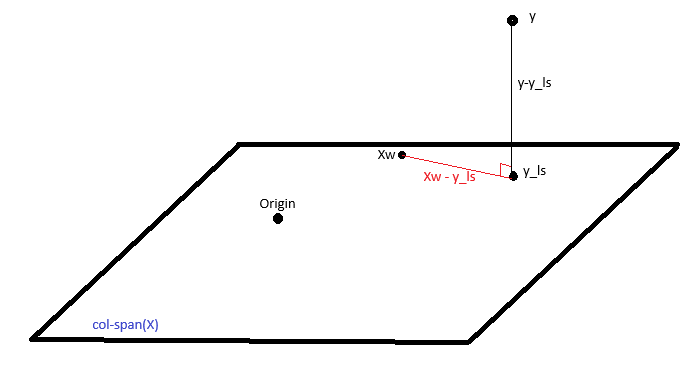
\includegraphics[scale=0.5]{./fig/geo.png}
			\end{center}
		\end{figure}
	\end{answer}
	\end{question}
	
	
\end{question}
\end{document}